\chapter{Regularisation and the Interpretation of CCA Weights and Loadings}\label{chap:als}
\minitoc

This chapter is an extension of work that I have previously presented in poster form at the OHBM conference and is
loosely related to a tutorial paper that I was a co-author on \cite{mihalik2022canonical} to which I contributed the
simulated data.

\section{Introduction}\label{sec:introduction}

This chapter explores the role of regularization in improving the performance and interpretation of Canonical
Correlation Analysis (CCA) using simulated and real data from the Human Connectome Project (HCP).

The application of Canonical Correlation Analysis (CCA) methods to practical problems often involves two key aspects: predicting latent variables associated with different views, and understanding the nature of the relationship between these views.
This dichotomy in goals bears resemblance to the distinction between machine learning and probabilistic or statistical approaches to the CCA problem.
Machine learning approaches prioritize (out-of-sample) prediction of latent variables for downstream tasks, while statistical approaches seek to infer the data generation process from latent variables to the observed data.
Notably, the probabilistic approach to CCA focusses on the forward model from latent variables to observed data, while the machine learning approach focusses on the inverse model from observed data to latent variables.
As a result the probabilistic CCA is parameterized by the \textit{loadings}, while the machine learning approach is parameterized by \textit{weights}.
We would ideally like to have the best possible prediction of the latent variables, while also being able to interpret the model and understand therelationship between the views.

In addition, CCA models often exhibit shortcomings when grappling with high-dimensional data, a challenge particularly acute in the context of brain-behavior studies with neuroimaging modalities typically having much higher dimensionality than the available sample size.
In this context, CCA models are prone to overfitting, leading to spurious correlations and poor generalization.
Regularization is a powerful tool for addressing linear models with extensive theory for Linear Regression and Inverse Problems.
Regularization can help us avoid overfitting and improve the interpretability of the results.

This chapter gives a new perspective on the relationship between the machine learning and probabilistic approaches to CCA. Through use of experiments with simulated data, we show that the approaches are not as distinct as they may seem.
We show that sparse regularization of CCA weights can give sparse estimates of the generative model loadings under certain conditions.
On the other hand we also show that sparse regularization of CCA weights does not necessarily imply sparse loadings, and that sparse regularized CCA models can be difficult to interpret under anisotropic noise.
We also show that regularization can improve model performance in low signal-to-noise ratio (SNR) settings but that resorting to the PLS objective (with or without regularization) can bias the model towards the largest principal components at the expense of more subtle correlations.

With this perspective in mind, we propose a flexible regularized alternating least squares (FRALS) framework for CCA which allows us to incorporate any regularized least squares solver to efficiently implement a wide range of regularization functions, but in particular allows us to efficiently implement the elastic net with controllable L2 and L1 penalties so that we can control the bias towards the largest principal components while still encouraging sparsity in the weights.
This is in contrast to much of the previous work on sparse Brain-Behavior analysis which has used a PLS objective with lasso constraints (SPLS), which inherits a bias towards the largest principal components from PLS.

We apply FRALS to the Human Connectome Project (HCP) dataset, and show that it outperforms other CCA models in terms of out-of-sample canonical correlation.
We also show that the identified mode of variation is distinct from previous work which identified latent variables with loadings related to cognitive tests and negatively related to cigarette, tobacco or alcohol\cite{smith2015positive}.
FRALS has stronger correlations with the Line Orientation test, which measures visuospatial abilities, and the parietal lobe, which is known to be involved in visuospatial processing.
This further demonstrates the importance of matching the model to the data generation process with the appropriate regularization.

\section{Background}\label{sec:background}

To understand how to interpret the weights of CCA models and therefore how to regularize the CCA problem, we first review probabilistic and generative perspectives on CCA. Then we review previous work on regularized CCA with a focus on ridge (L2), lasso (L1), and elastic net (L1 + L2) regularization.

\subsection{Generative Perspectives on CCA}
Understanding the data generation process in Canonical Correlation Analysis (CCA) and Partial Least Squares (PLS) is pivotal for many reasons.
It influences the choice of appropriate models, evaluation metrics, and sheds light on the underlying structure and dependencies between views.
Probabilistic formulations provide a principled framework to understand this process, helping us gauge the assumptions we make and the limitations these impose.

\subsubsection{A probabilistic latent variable perspective on CCA}

Consider the graphical model depicted in Figure \ref{fig:mentalhealthselfsupervised}.
It comprises two distinct views: a neuroimaging modality and a behavioral modality.
Both views are assumed to originate from a common latent variable, representing the severity of a mental health condition.
The neuroimaging modality is generated via a linear model with added noise, while the behavioral modality similarly arises from a linear model with noise.
Consequently, the brain and behavioral modalities exhibit correlation since they both derive from the same latent variable.
In a statistical sense, they are conditionally independent, given the latent variable.

\begin{figure}
    \centering
    \tikz{
        % nodes
        \node[latent, align=center, minimum size=2cm] (Z) {Severity\\(z)};
        %
        \node[obs, below left=of Z, minimum size=2cm] ($x\sps{1}$) {Brain\\($x\sps{1}$)};%
        \node[obs, below right=of Z, minimum size=2cm] ($x\sps{2}$) {Behaviour\\($x\sps{2}$)};%
        % edges
        \edge{Z} {$x\sps{1}$}
        \edge{Z} {$x\sps{2}$}}
    \caption[Latent Variable Model of Mental Health]{\textit{\textbf{Latent Variable Model of Mental Health:}} From this perspective the neuroimaging modality and behavioural data are both considered to have been generated with distributions conditioned on the severity of a mental health condition}\label{fig:mentalhealthselfsupervised}
\end{figure}

The distributions of the two views are given by:

\begin{align}
    z& \sim \mathcal{N}(0, I)\\
    x\sps{i} & \sim \mathcal{N}(W\sps{i} z + \mu\sps{i}, \Psi\sps{i})
\end{align}

Where \(z\) represents the latent variable (disease severity), \(x\sps{i}\) represents the $i^{\text{th}}$ view, \(W\sps{i}\) represents the model loadings, \(\mu\sps{i}\) represents the mean, and \(\Psi\sps{i}\) represents the noise covariance matrix for the $i^{\text{th}}$ view. 
Notice that if it were not for the view-specific noise, the two views would be perfectly correlated subject to a linear transformation.

\cite{bach2005probabilistic} showed that the maximum likelihood solution for this model is equivalent to the solution of the CCA problem in the sense that the loadings are the same as the CCA weights multiplied by the sample covariance:

\begin{align}\label{eq:probabilistic-cca}
    \hat{W}\sps{i} = \hat{\Sigma_{ii}} \hat{U}\sps{i} R
\end{align}

Where $R$ is an arbitrary rotation matrix and $\hat{U}\sps{i}$ is the matrix of CCA weights for the $i$th view.
This implies that for invertible covariance matrices, we can access the `true' CCA weights by multiplying the loadings by the inverse of the covariance matrix:

\begin{align}
    \hat{U}\sps{i} = \hat{\Sigma_{ii}}^{-1} \hat{W}\sps{i}
\end{align}

Notice that for Identity covariance matrices, the CCA weights are the same as the loadings.
Otherwise, there is a linear transformation between the two.
For singular covariance matrices, the CCA weights are not uniquely defined.

Moreover, the mean of the posterior distribution of the latent variables is proportional to the mean of the CCA scores\cite{klami2013bayesian}.
Group Factor Analysis (GFA) is a closely related model that assumes diagonal covariance in $\Psi\sps{i}$:

\begin{align}
    z& \sim \mathcal{N}(0, I)\\
    x\sps{i} & \sim \mathcal{N}(W\sps{i} z, \sigma\sps{i}I)
\end{align}

An interesting feature of the GFA model is that as the noise level approaches zero, the marginal distribution of the views is the same as the probabilistic PCA model for each view~\cite{tipping1999probabilistic}.
This suggests that for small noise levels, we should in fact be able to recover much of the mutual information between the views by using PCA on each view separately.
For this reason, we will use and recommend PCA as a baseline in our later experiments.
Because the diagonal covariance assumption makes inference computationally cheaper, this line of work has been able to extend to incorporate sparsity on the loadings\cite{virtanen2011bayesian} as well as missing data \cite{ferreira2022hierarchical}.

By marginalizing out the latent variables of the generative CCA and GFA models, we can write down the joint distribution of the two views:

\begin{align}
    \begin{bmatrix} X\sps{1} \\ X\sps{2} \end{bmatrix} \sim \mathcal{N} \left( \begin{bmatrix} \mu\sps{1} \\ \mu\sps{2} \end{bmatrix}, \begin{bmatrix} W\sps{1}W\spstop{1} + \Psi_1 & W\sps{1}W\spstop{2} \\ W\sps{2}W\spstop{1} & W\sps{2}W\spstop{2} + \Psi_2 \end{bmatrix} \right)
\end{align}

While these generative models are well-grounded in biological processes by the latent variable perspective, they are not applied as much as classical CCA in practice primarily because they are computationally expensive and require a careful choice of priors.
By selecting parameters for the generative model (rather than fitting them from data), we can generate data with known properties and in particular we can generate data with sparse loadings.
However this approach does not in general allow us to generate data with sparse weights, however, as the CCA weights are determined by the covariance matrices of the views.

\subsubsection{A Joint Covariance Matrix Perspective}

In order to generate data with sparse weights, we instead construct the joint covariance matrix\citep{mai2019iterative,chen2013sparse} of the two views as follows:

\begin{align}\label{eq:covariance}
    \begin{bmatrix} X\sps{1} \\ X\sps{2} \end{bmatrix} \sim \mathcal{N} \left( \begin{bmatrix} 0 \\ 0 \end{bmatrix}, \begin{bmatrix} \Sigma_{11} & \Sigma_{12} \\ \Sigma_{21} & \Sigma_{22} \end{bmatrix} \right)
\end{align}

Where $\Sigma_{11}$ and $\Sigma_{22}$ are the within-view covariance matrices and $\Sigma_{12}$ and $\Sigma_{21}$ are the between-view covariance matrices.

This has the advantage of allowing us to control the within-view covariance and therefore test the methods under specific conditions.
The process was first described by Chen~\cite{chen2013sparse} and further explained by~\cite{suo2017sparse}.

We can control the true signal by setting the active variables and correlations in the between-view covariance matrices $\Sigma_{12}$ and $\Sigma_{21}$.
Specifically we construct the between-view covariance matrices as follows:

\begin{align}
    \Sigma_{12}=\sum_{k=1}^{K}\rho_k\Sigma_{11}u\sps{1}_{k}u\spstop{2}_k\Sigma_{22}
\end{align}

Where $\rho_k$ is the $k^{\text{th}}$ canonical correlation and $u\sps{i}_k$ is the $k^{\text{th}}$ column of the matrix of weights $U\sps{i}$.

We can still access the true loadings of the implied latent variable model by using the relationship in \ref{eq:probabilistic-cca} and multiplying the weights $u\sps{i}$ by the within-view covariance matrix $\Sigma_{ii}$.

\subsubsection{Summary of Data Generation Methods}

We summarise the joint covariance matrices of each of the data generation methods we have described in table \ref{table:data-generation-methods}.
This

\begin{table}[h]
    \centering
    \caption{Summary of Data Generation Methods}
    \begin{tabular}{|l|c|}
        \hline
        Method & Within-view Covariance \Sigma_{ii} & Covariance \Sigma{12}  \\
        \hline
        Probabilistic CCA &
        W\sps{i}W\spstop{i} + \Psi_i & W\sps{1}W\spstop{2} \\

        Probabilistic CCA (Diagonal) &
        W\sps{1}W\spstop{1} + \sigma\sps{1} I & W\sps{1}W\spstop{2} \\

        Joint Covariance &
        \Sigma_{ii} & \sum_{k=1}^{K}\rho_k\Sigma_{11}u\sps{1}_{k}u\sps{2\top}_k\Sigma_{22} \\
        \hline
    \end{tabular}
    \label{table:data-generation-methods}
\end{table}

These models give rise to different properties in the data, which we summarise in table \ref{table:data-generation-methods-properties}.

\begin{table}[h]
    \centering
    \caption{Summary of Data Generation Methods}
    \begin{tabular}{c|c|c|c|c|}
        \hline
        \textbf{Method} & \textbf{\Sigma_{ii}} & \textbf{Sparse Weights}& \textbf{Sparse
        Loadings} & \text{True Correlation} \\
        \hline
        Probabilistic CCA & Implied& No& Controlled&Implied\\
        GFA & Implied& No& Controlled&Implied\\
        Joint Covariance& Controlled  & Controlled& No&Controlled\\
        \hline
    \end{tabular}
    \label{table:data-generation-methods-properties}
\end{table}

Now that we have a clear understanding of data generation methods, we shift our focus to the importance of regularization in handling high-dimensional and structured data.

\subsection{Regularisation for High-Dimensional and Structured Data}

Like Linear Regression, Canonical Correlation Analysis does not have a unique solution when the number of features exceeds the number of observations in either view.
More generally, as the number of features increases, the number of parameters in the model increases, and the model becomes more prone to overfitting particularly when the signal-to-noise ratio is low.
Furthermore, when features are correlated, the estimates of the parameters become unstable.
Most obviously, if two features are perfectly correlated, the model is not identifiable because we can swap the weights between the two features without changing the model.
Regularization is a powerful tool for addressing these problems, and has been widely used in Linear Regression and Inverse Problems.
Moreover, regularization can help us improve the interpretability of the results by encouraging sparsity in the weights and/or loadings.

\subsubsection{Shrinkage Regularization}

Shrinkage regularization is an effective method for improving the performance of linear models in high-dimensional settings.
Shrinkage methods bias models towards lower variance solutions by shrinking the model parameters (weights) towards zero.
Shrinkage regularization works on the premise that, generally, larger principal components are more likely to represent meaningful data patterns rather than noise.

\paragraph{PLS as Shrinkage Regularization}

PLS can be interpreted as a form of shrinkage regularization applied to CCA. We can explain this by considering an analogy between CCA and Linear Regression (indeed Linear Regression is a special case of CCA where \(X^{(2)}\) has one feature).

In Linear Regression, the ridge regression solution is given by:
\begin{align}
    \hat{\beta}_{\text{ridge}} = ((1-\lambda)\Sigma_{X,X} + \lambda I)^{-1} \Sigma_{X,y}
\end{align}
Where \(\lambda\) is the regularization parameter between 0 and 1. The ridge penalty acts in two important ways:
\begin{itemize}
    \item It shrinks the weights towards zero.
    \item It biases the solution to high covariance directions rather than high correlation directions.
\end{itemize}

As $\lambda$ becomes large, $\lim_{\lambda \to \infty} (\Sigma_{X,X} + \lambda I)^{-1} = (\lambda I)^{-1}$
, so that $\hat{\beta}_{\text{ridge}}=\frac{\Sigma_{X,y}}{\lambda}$, which is precisely the covariance of the features of $X$ with $Y$ scaled by $\lambda$ (and shrunk towards zero for $\lambda \geq 1$).
Notice that the ridge regression solution is no longer sensitive to the correlation of features in $X$.
Additionally, notice that for sufficiently large $\lambda$, $(\Sigma_{X,X} + \lambda I)$ is invertible even if $\Sigma_{X,X}$ is not invertible, so that ridge regression can be well defined even when the number of features exceeds the number of observations.

Now consider the CCA problem.
Firstly, recall that PLS and CCA are equivalent up to a scaling when the covariance matrices are identity matrices, a similar relationship to the relationship between Linear and Ridge Regression.
Consider the form of CCA given in equation \ref{eq:cca}:

\begin{align}\label{eq:cca}
     & u_{\text{opt}}=\underset{u}{\mathrm{argmax}}\{ u\spstop{1}(\Sigma_{11}+ c_1 I)^{-\frac{1}{2}}\Sigma_{12}(\Sigma_{22}+c_2 I)^{-\frac{1}{2}}u\sps{2} \} \\
     & \text{subject to:} \notag \\
     & u\spstop{1}u\sps{1}=1, u\spstop{2}u\sps{2}=1 \notag
\end{align}

As we increase $c_1$ and $c_2$, $\lim_{c_i \to \infty} (\Sigma_{ii}+ c_i I)^{-\frac{1}{2}}= (c I)^{-1}$ so that the objective approaches:

\begin{align}\label
     & u_{\text{opt}}=\underset{u}{\mathrm{argmax}}\{ u\spstop{1}(c_1 I)^{-1}\Sigma_{12}(c_2 I)^{-1}u\sps{2} \} \\
        & \text{subject to:} \notag \\
        & u\spstop{1}u\sps{1}=1, u\spstop{2}u\sps{1}=1 \notag
\end{align}

Which is precisely the PLS objective and constraints with an arbitrary scaling of the covariance matrix $\Sigma_{12}$.
For this reason, we can consider PLS as a shrinkage method for CCA equivalent to adding a very large ridge regularization.
This has two important consequences: firstly, it biases the solution towards the largest principal components, and secondly, it is well defined even when the number of features exceeds the number of observations.
However, PLS is not a nuanced as a tool for regularization because it offers limited control over the degree of regularization applied.

\paragraph{Ridge Regularisation}

Vinod proposed the 'Canonical Ridge' which combined the PLS and CCA constraints in a single constrained optimisation~\cite{vinod1976canonical}:

\begin{align}
     & u\sps{1}_{\text{opt}} = \underset{u\sps{1}}{\mathrm{argmax}} \{ u\spstop{1} \hat{\Sigma_{12}} u\sps{2} \} \\
     & \text{subject to:} \notag \\
     & (1 - c_1) u\spstop{1} \hat{\Sigma_{11}} u\sps{1} + c_1 u\spstop{1} u\sps{1} = 1 \notag \\
     & (1 - \tau_2) u\spstop{2} \hat{\Sigma_{22}} u\sps{2} + \tau_2 u\spstop{2} u\sps{2} = 1 \notag
\end{align}

And this gives us the generalized eigenvalue problem~\cite{rosipal2005overview}:

\begin{align}
    \begin{pmatrix}
        0 & \hat{\Sigma_{12}} \\
        \hat{\Sigma_{21}} & 0 
    \end{pmatrix} \begin{pmatrix}
        u^{(1)} \\
        u^{(2)}
    \end{pmatrix}= \begin{pmatrix}
        (1-c_1)\hat{\Sigma_{11}} + c_1I \\
        0 & (1-c_2)\hat{\Sigma_{22}} + c_2I
    \end{pmatrix}\begin{pmatrix}
        u^{(1)} \\
        u^{(2)}
    \end{pmatrix}
\end{align}

The main difference between this eigenvalue problem and the CCA eigenvalue problem is the substitution of the matrices \(\Sigma_{11}\) and \(\Sigma_{22}\) for the matrices \( ((1-c_1) \Sigma_{11} + c_1 I) \) and \( ((1-c_2) \Sigma_{22} + c_2 I) \).
We can therefore see that this regularisation is equivalent to adding a constant `ridge' to the diagonal of the covariance matrix \(X\spstop{i} X\sps{i}\).

\paragraph{PCA-CCA}

PCA-CCA can be used as a regularisation method for CCA by using only the first \( k \) principal components of each view as the input to CCA.
This reduces the dimensionality of the data and can help to avoid overfitting.
However, it also risks overlooking subtle but crucial relationships between variables, as it focuses on leading principal components.

While PCA-CCA and rCCA are effective for finding signal in the presence of noise, they do not produce sparse
solutions and so do not clearly lend themselves to interpretation.

\paragraph{Visual Comparison of Shrinkage Techniques}

The distinct effects of Ridge and PCA on the eigenvalues of the effective covariance matrices can be clearly visualized.
As shown in Figure \ref{fig:shrinkage}, Ridge regularization uniformly reduces the magnitude of all principal components towards zero, with a proportionally greater effect on the smaller components.
On the other hand, PCA-CCA, by focusing on leading principal components, only shrinks the smallest ones.

\begin{figure}[htbp]
    \centering
    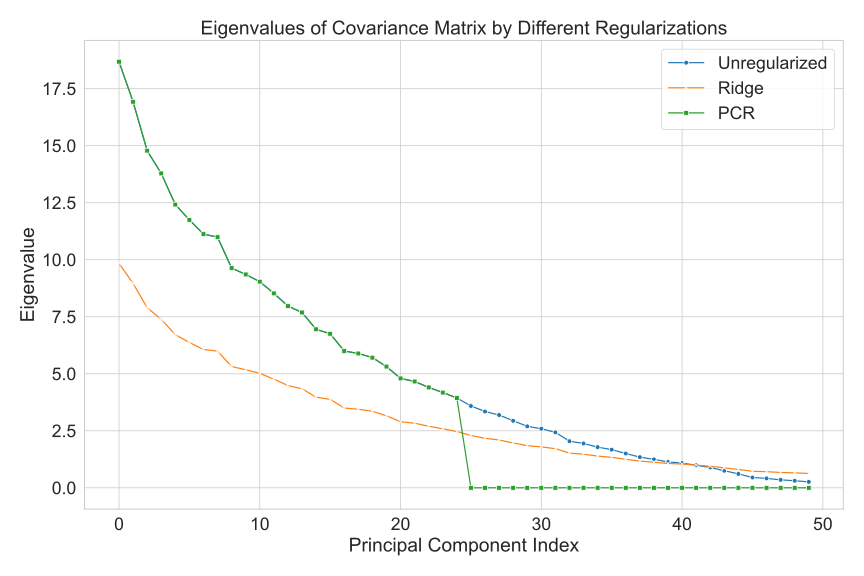
\includegraphics[width=0.8\textwidth]{figures/regularisation/shrinkage/shrinkage.svg}
    \caption{Comparison of the effect of OLS, Ridge, and PCA-CCA regularization on the eigenvalues of the covariance matrix.}
    \label{fig:shrinkage}
\end{figure}

The visualization underscores the intrinsic nature of each regularization method:
\begin{itemize}
    \item \textbf{Unregularized}: Presents the unaltered spectrum, making it susceptible to noise but preserving potential subtle patterns.
    \item \textbf{Ridge}: Applies consistent shrinkage across all components, reducing noise but possibly attenuating genuine signal.
    \item \textbf{PCA}: Focuses on dominant patterns by shrinking smaller components, potentially missing subtle connections but offering a cleaner representation of strong associations.
\end{itemize}
The choice between these shrinkage techniques should in general be based on the nature of the data.
We now transition to another essential regularization technique: sparse regularization.
While shrinkage aims to prevent overfitting by pulling weight estimates towards zero to reduce variance, sparse regularization aims to set weights to zero with the added benefit of enhancing model interpretability.

\subsubsection{Sparse Regularization}

Sparse regularization is a powerful tool for improving the performance and interpretability of linear models.
Sparse regularization encourages the model to use only a subset of the features, which can help to avoid overfitting and improve the interpretability of the model.
Sparse regularization works on the premise that only a subset of the features are relevant to the model.
Sparsity is typically achieved by adding either an L1 penalty or constraint \footnote{The L0 norm of the weight vector is the number of non-zero elements in the vector and is arguably a closer match to the goal, but the L0 norm is a) not a proper norm in the mathematical sense and b) not convex and so is difficult to optimize.}.
The L1 penalty is defined as:

\begin{align}
    \|u\|_1 = \sum_i |u_i|
\end{align}

Intuitively, this is the sum of the absolute values of the elements of the vector.
Now, with a foundational understanding of sparse regularization, we review a number of approaches to adding sparsity to the CCA problem.

\paragraph{Sparse PLS: Penalized Matrix Decomposition}
Penalized Matrix Decomposition (PMD) \cite{witten2009penalized} provides an approximate solution to the sparse CCA problem by altering the constraints of the classical CCA formulation.
Specifically, PMD replaces the constraint \(u\spstop{1} \hat{\Sigma_{11}} u\sps{1} = 1\) with \(u\spstop{1} u\sps{1} \leq 1\).
The optimization problem for PMD is then given by:

\begin{align}
    & u^{opt}=\underset{u}{\mathrm{argmax}}\{ u\spstop{1} \hat{\Sigma_{12}} u\sps{2} \} \\
    & \text{subject to:} \notag \\
    & u\spstop{1} u\sps{1} \leq 1 , u\spstop{2} u\sps{2} \leq 1 \notag \\
    & P(u\sps{1}) \leq c_1 , P(u\sps{2}) \leq c_2 \notag
\end{align}

Despite its influence, this method effectively performs Sparse PLS (SPLS) rather than Sparse CCA as in the original work.
For this reason, we refer to this method as SPLS in the rest of this thesis.
There are a number of other sparse CCA methods that employ a similar assumption to SPLS\cite{parkhomenko2009sparse, waaijenborg2008quantifying}.

While SPLS is an extremely efficient method (it can be solved by iteratively multiplying $u\sps{1}$ by $\hat{\Sigma_{12}}$ and soft thresholding), it is clear that it is not always a good approximation to the sparse CCA problem.

A number of approaches to Sparse CCA instead adopt a penalized least squares approach.

\paragraph{Sparse CCA: Least Squares Approaches}

It is well known that the CCA problem can be formulated as a constrained least squares problem with the intuition that
for unit norm \(X\sps{1} u\sps{1}\) and \(X\sps{2} u\sps{2}\), correlation is maximized when the squared distance
between \(X\sps{1} u\sps{1}\) and \(X\sps{2} u\sps{2}\) is minimized. \cite{golub1995canonical} proved the
convergence of a simple algorithm which alternates between solving the least squares problem for \(u\sps{1}\) and
\(u\sps{2}\) while keeping the other fixed.

With this intuition, \cite{wilms2015sparse} and \cite{mai2019iterative} separately proposed iterative penalized least
squares methods for sparse CCA.

\begin{align}
    \label{eq:mai}
    u^{opt} &= \underset{u}{\mathrm{argmin}} \left\{ \|X\sps{1}u\sps{1} - X\sps{2}u\sps{2}\|_2^2 + P(u) \right\} \\
    &\text{subject to:} \notag \\
    &u\spstop{1} \hat{\Sigma_{11}} u\sps{1}=1 \notag \\
    &u\spstop{2} \hat{\Sigma_{22}} u\sps{2}=1 \notag
\end{align}

Where \(P(u)\) is a penalty function.
The penalty term can be any function that penalizes the norm of the vector \(u\).
\cite{mai2019iterative} proved that solving the subproblems where one of $u\sps{i}$ is fixed is easy for one-homogenous $P$ where
\( P((\mu + 1)\theta) = (\mu + 1)P(\theta) \) which notably includes the lasso penalty.
This means a sparse CCA based
on alternating lasso regressions can be solved relatively efficiently using existing solvers.
However, the one homogenous penalty in practice limits the flexibility of the method.
For example, the elastic net penalty is not one-homogenous and therefore cannot be used with this method.\cite{
    kanatsoulis2018structured} proposed solving equation \ref{eq:mai} for more general classes of $P$ using the
alternating direction method of multipliers (ADMM) \cite{boyd2011distributed}.

Finally, the closest method to ours is the sparse CCA method proposed by \cite{fu2017scalable} which uses an
alternative classical formulation of the CCA problem as a constrained least squares problem\cite{
    carroll1968generalization,
    kettenring1971canonical}:

\begin{gather*}
    \underset{U, T}{\mathrm{argmin}}\left\{\sum_i \|X\sps{i} U\sps{i} - T\|_F^2 \right\}\\
    \text{subject to: }T^\top T = I\\
\end{gather*}

Where \(U\sps{i}\) is the matrix of weights for the $i^{\text{th}}$ view and \(T\) is the matrix of latent variables. This
approach has the benefit of being extendable to more than two views. The authors proposed to solve this problem using
proximal gradient descent for penalties with a closed form proximal operator, such as the lasso penalty.

In this section, we have illustrated the benefits of shrinkage regularization (PCA-CCA, Ridge CCA, PLS) and sparse regularization (SPLS and Sparse CCA) for handling noisy and high-dimensional data with parsimonious solutions.
In this chapter, we turn our attention to the problem of incorporating both tunable shrinkage and sparsity into the CCA problem for Brain-Behaviour associations.

\section{Methods}

In this section, we outline the methodologies employed in our study for Canonical Correlation Analysis (CCA) and related techniques.
We begin with a description of Flexible Regularized Alternating Least Squares (FRALS), a versatile approach to solve the CCA problem.
Following that, we discuss the experiment design, including data splitting, model selection, and comparisons.
Additionally, we detail the generation of both simulated and real datasets used in our experiments, shedding light on their parameters and sources.
This section serves as a comprehensive guide to the techniques and procedures underpinning our investigation.

\subsection{Flexible Regularized Alternating Least Squares (FRALS)}\label{subsec:flexible-regularized-alternating-least
-squares-(frals)}

We adopt an alternating minimization strategy to solve the CCA problem.
The objective is to minimize the sum of squared Frobenius norms between the latent variables and their projections in each view.
Regularization terms are added to the objective function to avoid overfitting.
Our formulation allows the incorporation of any regularized least squares solver, making it extremely flexible.

\subsubsection{Mathematical Formulation}
We can solve CCA by alternating minimization over each view, based on the alternating least squares form.
This form finds a variable \( T \) that is close to the latent variables \( X\sps{1} U\sps{1} \).
The closer \( T \)is to\( X\sps{1} U\sps{1} \), the higher the correlation between them.
The constraint \( T^\top T = I \)ensures that the latent space is orthogonal.

\begin{gather*}
    \underset{U, T}{\mathrm{argmin}}\left\{\sum_i \|X\sps{i} U\sps{i} - T\|_F^2 \right\}\\
    \text{subject to: }T^\top T = I\\
\end{gather*}

To regularize the projection matrices, we add penalty terms to the objective function, such as \( P(U\sps{i}) = \lambda_i \|U\sps{i}\|_F \)for ridge regression or \( P(U\sps{i}) = \lambda_i \|U\sps{i}\|_1 \) for lasso.
This can help us avoid overfitting and improving the interpretability of the results.
This means that \textbf{any regularized least squares solver} can be used to solve each subproblem, such as ridge regression, lasso, elastic net, etc., making our framework substantially more flexible than prior work.

\begin{gather*}
    \underset{U, T}{\mathrm{argmin}}\left\{\sum_i \|X\sps{i} U\sps{i} - T\|_F^2 + \textcolor{red}{\lambda_i P(U\sps{i})}\right\}\\
    \text{subject to: }T^\top T = I\\
\end{gather*}

In practice, we use the high quality and well tested implementations of regularized least squares solvers in the \texttt{scikit-learn} package \cite{pedregosa2011scikit}.

\subsection{Experiment Design}

\subsubsection{The predictive framework for CCA}

In order to evaluate the performance of CCA models, we employ a standard predictive framework.
We split the data into training and test sets, and use the training set to fit the model.
We then use the test set to evaluate the model's performance.

\subsubsection{Model Selection}

For the models that require hyperparameter tuning, we use a grid search to find the best hyperparameters.
Specifically, we use 5-fold cross-validation to evaluate the performance of a model with a given set of
hyperparameters on 5 different splits of the training data with non-overlapping validation sets. We optimise for the
hyperparameters that give the best average out of sample correlation.

\subsubsection{Model Comparisons}
We employ several CCA variants for this experiment, including Canonical Correlation Analysis (CCA), Partial Least Squares (PLS), and more.
Grid search is employed for hyperparameter tuning.

\begin{table}[h]
\centering
\caption{Employed CCA Variants}
\begin{tabular}{|l|l|l|l|}
\hline
\textbf{Model} & \textbf{Abbreviation} & \textbf{Hyperparameters} & \textbf{Objective} \\
\hline
Canonical Correlation Analysis & CCA & - & Correlation \\
\hline
Regularized CCA & RCCA & \(c_1, c_2\) & Correlation \\
\hline
Partial Least Squares & PLS & - & PLS \\
\hline
Sparse PLS & SPLS & \(\tau_1, \tau_2\) & PLS \\
\hline
FRALS - Elastic & Elastic & \(c_1, c_2, \text{l1}_1, \text{l1}_2\) & Correlation \\
\hline
Principal Component Analysis & PCA & - & PCA \\
\hline
PCA-based Canonical Correlation Analysis & PCA-CCA & - & Correlation \\
\hline
\end{tabular}
\label{table:cca-variants}
\end{table}

\subsection{Data}

\subsubsection{Simulated Data}

In order to investigate the performance of models and the effect of regularisation on the CCA loadings and weights,
we generated simulated data with known properties. We used a true population canonical correlation of 0.99, and
generated data with 1000 observations and 1000 variables in each view. We generated

\textbf{Sparse Weights:}

In order to generate data with sparse weights, we used the joint covariance method described in section \ref{subsec
:joint-covariance}. We compare the case where the covariance matrices are identity matrices such that the true weights
are also the true loadings, and the case where the covariance matrices are not identity matrices such that the true
weights are not the true loadings (and are in general not sparse).

\textbf{Sparse Loadings:}

In order to generate data with sparse loadings, we used the probabilistic CCA model described in section \ref{subsec
:probabilistic-cca-rcca-and-pls}. We compare the case where the noise covariance matrices are identity matrices such
that the true weights are also the true loadings, and the case where the noise covariance matrices are not identity matrices
such that the true weights are not the true loadings (and are in general not sparse).

\begin{table}[h]
\centering
\caption{Simulated Data Parameters}
\begin{tabular}{| l | l |}
\textbf{Parameter} & \textbf{Value} \\
Number of samples (\textit{n}) & 500 \\
Number of features in View 1 (\textit{p}) & 200 \\
Number of features in View 2 (\textit{q}) & 200 \\
True Latent dimensions & 1 \\
Sparsity in View 1 & 0.1 \\
Sparsity in View 2 & 0.1 \\
\end{tabular}
\end{table}


\subsubsection{Real Data}

The real datasets employed in our experiments comprise the HCP and ADNI data. These datasets provide insights into brain functionality and behavior from different perspectives.
We chose the HCP and the ADNI datasets based on 2
recent landmark studies and the tutorial paper this chapter is loosely related to \cite{mihalik2022canonical}. 


The Human Connectome Project (HCP) offers publicly available resting-state functional MRI (rs-fMRI) and non-imaging
measures like demographics, psychometrics, and other behavioral measures.
Specifically, we sourced data from 1003
subjects out of the 1200-subject data release of the HCP (\url{https://www.humanconnectome.org/study/hcp-young-adult/data-releases}). This dataset is constructed using brain connectivity features of the thoroughly processed rs-fMRI data. This processing results in 19,900 brain variables for every subject. Additionally, there are 145 non-imaging measures employed. Notably, nine confounding variables were regressed out from both data modalities. Each variable was standardized for zero mean and unit variance. More details can be found in \cite{smith2015positive, mihalik2022canonical}.

\begin{table}[h]
\centering
\caption{HCP Data Parameters}
\begin{tabular}{| l | l |}
\hline
\textbf{Parameter} & \textbf{Value} \\
\hline
Number of samples (\textit{n}) & 1001 \\
Number of features in View 1 (\textit{p}) & 19900 \\
Number of features in View 2 (\textit{q}) & 145 \\
\hline
\end{tabular}
\label{table:hcp-parameters}
\end{table}

\textbf{ADNI Data:}
The Alzheimer’s Disease Neuroimaging Initiative (ADNI) database is found at \url{adni.loni.usc.edu}.
Launched in 2003, ADNI's main objective is to assess the combination of serial MRI, PET, biological markers, and clinical and neuropsychological assessment in tracking the progression of MCI and early Alzheimer’s disease.
For our experiments, we used a subset of 592 unique subjects from the ADNI. The MRI scans underwent a series of processing stages, yielding a grey matter probability map.
The Mini-Mental State Examination (MMSE) scores were employed to investigate the association with the grey matter maps.

\begin{table}[h]
\centering
\caption{ADNI Data Parameters}
\begin{tabular}{| l | l |}
\hline
\textbf{Parameter} & \textbf{Value} \\
\hline
Number of samples (\textit{n}) & 592 \\
Number of features in View 1 (\textit{p}) & 168130 \\
Number of features in View 2 (\textit{q}) & Varied (MMSE scores) \\
\hline
\end{tabular}
\label{table:adni-parameters}
\end{table}

\section{Results}

\subsection{Simulated Data}

\subsubsection{Sparse Weights only Imply Sparse Loadings when Within-View Covariance Matrices are Diagonal Matrices}

While obvious from the theory, the figures show that the weights of the bac

\subsubsection{}

In the low dimensional case, we found that

\subsubsection{High Dimensional Data}


\subsection{Regularized CCA with the Human Connectome Project (HCP) Data}

FRALS outperformed the other models by achieving the highest out-of-sample canonical correlations (Figure~\ref{fig:performance}).

\begin{figure}[h]
\centering
\includesvg[width=0.5\linewidth]{figures/regularisation/hcp/barcorr}
\caption{Out-of-sample canonical correlations for each model.}
\label{fig:performance}
\end{figure}

\subsubsection{Model Similarities}
We computed the correlation matrix of scores for each modality to assess how similar the latent variables were across models. FRALS showed low or negative correlations with other models (Figure~\ref{fig:similarities}).

\begin{figure}[h]
\centering
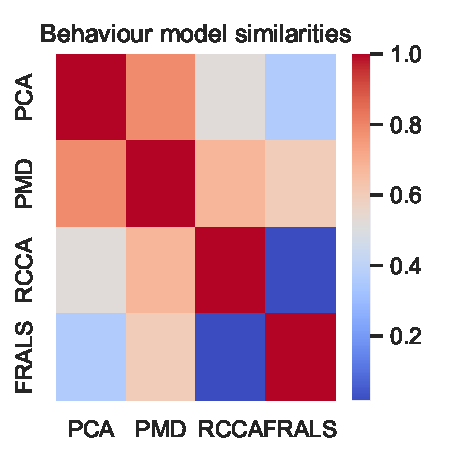
\includegraphics[width=0.49\linewidth]{figures/regularisation/hcp/behaviour_model_similarities}
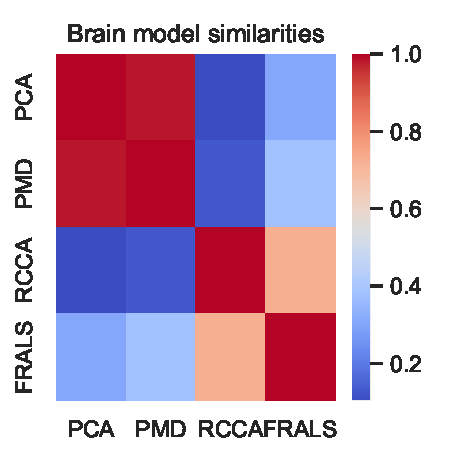
\includegraphics[width=0.49\linewidth]{figures/regularisation/hcp/brain_model_similarities}
\caption{Left: Correlation matrix of scores for each modality. Right: Correlation matrix of brain loadings for each model.}
\label{fig:similarities}
\end{figure}

\subsubsection{Behaviour and Brain Loadings}
All models, except PCA, identified a latent variable that had a positive correlation with cognitive tests and a negative correlation with cigarette, tobacco, or alcohol use. Both RCCA and FRALS correlated more strongly with the Line Orientation test.

\begin{figure}[h]
\centering
\includesvg[width=\linewidth]{figures/regularisation/hcp/all_top_and_bottom_loadings.svg}
\caption*{Top 5 positive and negative non-imaging loadings for each model}
\label{fig:behaviour}
\end{figure}

Regarding brain loadings, models assigned different weights to various brain regions based on their connectivity.

\begin{figure}[h]
\centering
\includegraphics[width=0.49\linewidth]{figures/regularisation/hcp/pca_brain_loadings}
\includegraphics[width=0.49\linewidth]{figures/regularisation/hcp/pmd_brain_loadings}
\includegraphics[width=0.49\linewidth]{figures/regularisation/hcp/rcca_brain_loadings}
\includegraphics[width=0.49\linewidth]{figures/regularisation/hcp/flexals_brain_loadings}
\caption*{Map of CCA connection strength variations, with each node’s parcel map weighted by CCA edge-strength changes across edges involving that node.}
\label{fig:brain}
\end{figure}

\section{Discussion and Limitations}

\subsection{Discussion}

\subsubsection{Structured regularisation makes sense when noise is isotropic}

\subsubsection{The importance of matching the model to the data generating process}

\subsubsection{FRALS allows for flexible regularisation for closer model matching}

\subsubsection{FRALS finds a subtly different mode to other models in the HCP data}

RCCA and FRALS gave more weight to the parietal lobe than PCA and PMD did.
This suggests that our model finds the parietal lobe more relevant for capturing brain-behaviour correlations.
PMD focused on principal components in the brain.
This could mean PMD might miss the true associations between views.
In this setting, FRALS functions similarly to a sparse RCCA.

\subsection{Limitations}
While FRALS offers promising performance in terms of out-of-sample correlation, it does come with significant drawbacks, the most noteworthy being its computational inefficiency.
Below, we outline the primary factors contributing to the slow speed of FRALS and provide some insights into the computational bottlenecks.

\subsubsection{Computational Time}\label{subsec:computational-time}
While computationally intensive, the flexibility of FRALS allows it to adapt better to the complexity inherent in real-world data sets, such as the HCP. This adaptability could be crucial when high predictive accuracy or interpretability is required.

\subsubsection{Changing Regression Targets}\label{subsec:changing-regression-targets}
Adding to the computational burden is the fact that the regression targets, i.e., the projections of the other view, are not static but change dynamically throughout the algorithm's run.
Each update to the least squares solution consequently alters the global objective, leading to a constantly shifting landscape that the algorithm needs to navigate.

\section{Conclusions}
In this chapter, we explored the relationship between the backward and forward models of CCA. We found that the weights of the backward model don't always imply sparsity in the forward model loadings. We proposed that inferring the loadings could provide more biologically relevant insights.

To enhance CCA model regularisation, we introduced the idea of using elastic net regularisation.
We developed a model using alternating least squares to incorporate this regularisation method.

Using simulated data, we discovered that when noise is isotropic with diagonal covariance, weights and loadings in the CCA model are equivalent.
We also compared CCA and PLS, finding that CCA performs better in high noise environments with large sample sizes,
while PLS can preferable for small sample sizes.

In real Brain-Behaviour data from the Human Connectome Project, we showed that some regularised CCA models can have significant model mismatches, leading to reduced performance in out-of-sample correlation.

Overall, our findings emphasize the importance of understanding and selecting the appropriate model for specific data scenarios.



